\section{Everyone Who Wants to Do Constraint Satisfaction Always Ends in Universal Problems}
% Everyone who wants to do good to the human race always ends in universal bullying.
% - Aldous Huxley

\begin{marginfigure}
	\centering
	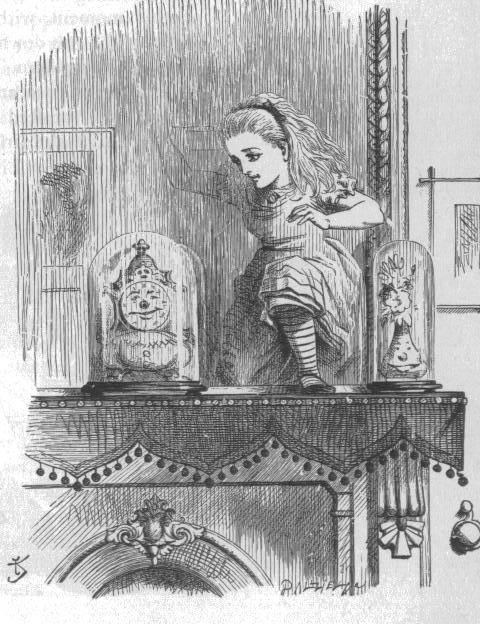
\includegraphics[width=\linewidth]{fig/intro/aliceroom2.jpg}
	\caption{Looking glass room, by John Tenniel.}
\end{marginfigure}

Going to the other side, encodings of model-checking problems
as "homomorphism problems" of the form $\textsf{data} \homto^? \textsf{query}$
can be thought of as ``universal problems'':%
\footnote{Here ``universal'' does not
refer to some form of completeness, but simply to universal quantification.}
notice "eg" that they are anti-monotonic with respect to the data:
for all "structures" $\?A$, $\?A'$ and $\?B$, if $\?A \homto \?B$ and $\?A'$ is a substructure
of $\?A$ then $\?A' \homto \?B$.
Moreover, while problems of the form $\textsf{query} \homto^? \textsf{data}$
can be solved locally---whether a vertex of the data is part of a solution (a "homomorphism") only 
depends on its neighbourhood---, problems $\textsf{data} \homto^? \textsf{query}$ cannot.
For instance, "3-colourability" is a global property of a graph and cannot by gluing local 
solutions. In particular, this implies that fixing the query does not necessarily result in
a drop in the complexity: for instance SAT-solving and "3-colourability" are already "NP"-complete.

However not all of these problems are hard: $2$-colourability is not only polynomial-time,
but can be solved using a greedy algorithm. This begs the question of understanding what
makes a "relational structure" hard for the "homomorphism problem".
This question is not only motivated by theory: constraint logic programming has emerged in the 1980s
with Prolog II and III; today programming languages such as answer-set programming provide an 
efficient was of doing constraint solving.

\begin{figure}
	\centering
	\lstinputlisting[language=Prolog, breaklines=true]{fig/intro/sudoku.lp}
	\caption{
		\AP\label{fig:ex-sudoku-asp}
		A Clingo program (answer-set programming) to solve Sudoku grids.
		Written by Enrico Höschler
		\href{https://ddmler.github.io/asp/2018/07/10/answer-set-programming-sudoku-solver.html}{[source]}.
		Try running it on \url{https://potassco.org/clingo/run/}!
	}
\end{figure}

Answer-set programming can be thought of, albeit caricaturally, as a human-readable
SAT-solver. It deals with variables, relations between these variables,
and logical rules between these variables. These rules take the form
\lstinline|A :- B|, which can be understood as `if $B$, then $A$'.
The right-hand side is parsed conjunctively while the left-hand side is parsed disjunctively:
\lstinline|A, B :- C, D| should be understood as `if $C$ and $D$, then $A$ or $B$'.
\Cref{fig:ex-sudoku-asp} provides
an example of a Clingo program for solving Sudoku grids:
\begin{itemize}
	\item it starts by declaring three types of variables: absissa $x$, ordinates $y$ and entries $x$ (representing a value in the grid), as well as their range;
	\item it introduces a \textsf{sudoku} ternary relation, where $\textsf{sudoku}(x,y,n)$
		represents the fact that entry $(x,y)$ of the grid has value $n$,
		and it says that there should be exactly one value per entry;
	\item it introduces a \textsf{subgrid} relation, saying when too entries
		belong to the same 3*3-square;
	\item finally, it says that any two values on the same column, row or subgrid
		must be different.%
		\footnote{Recall that the left-hand side of rules is understood disjunctively,
		and hence \lstinline|:- A, B| reads as `if $A$ and $B$, then false'.}
\end{itemize}
To solve a specific grid using the program of \Cref{fig:ex-sudoku-asp},
it suffices to add declarations of the form \lstinline|sudoku(4,1,5).| to say that entry
at position $(4,1)$ has value 5.%
\footnote{\lstinline|A.| is a shorthand for \lstinline|A :-.|.}

Contrary to more classical programming languages, this paradigm does not explain \emph{how} things
should be computed, but \emph{what constraints} the memory/solution should satisfy.
In "homomorphism problems", the "target structure" precisely plays this role of
encoding constraints. For instance, the only constraint for a graph $3$-colouring is that
adjacent vertices must be mapped to distinct colours: this constraint is
reflected in $\clique{3}$ by the fact that the edges of $\clique{3}$ are exactly the pairs
of distinct colours.

The field of \emph{constraint satisfaction problems} precisely aims at classifying the
structures $\?B$ "wrt" to the complexity of the "homomorphism problem" when the
"target structure" is $\?B$. One of the earliest and most impactful result
of the domain as found by Schaefer \cite{Schaefer1978ComplexitySatisfiability},
who proved that such problems are either in "P" or "NP"-complete when the domain of $\?B$
has two elements.%
\footnote{While this might seem restrictive, notice that no assumption is made on the "signature".
Moreover, the example of SAT-solving (\Cref{ex:sat-as-hom}) precisely uses a "structure" of this kind.}
A decade later, Hell and Ne\v{s}et\v{r}il \cite{HellNesetril1990ComplexityColoring}
proved a similar result for undirected graph.
Moreover, in both cases, these dichotomies are effective: given a structure, we can decide if
its "homomorphism problem" is in "P" or is "NP"-complete.
These results, together with the importance of \emph{constraint satisfaction} in computer science
lead Feder and Vardi at the end of the 1990s
to state their infamous \emph{dichotomy conjecture}: ``for any "relational structure" $\?B$,
the "homomorphism problem" with "target structure" $\?B$ is either "P"
or "NP"-complete'' \cite{FederVardi1998ComputationalStructure}.
Despite receiving lots of attention, the conjecture remained wide open for two decades, until
Bulatov \cite{Bulatov2017DichotomyCSPs} and Zhuk \cite{Zhuk2020CSPDichotomy} independently
showed the conjecture to be true.

However not all problems in "P" are complete for this class: some are even simpler and are complete
for "NL" or "L", or even "FOfin"---the class of "first-order definable" "finite structures".
One result that will be of major importance in this thesis is a dichotomy
theorem by Larose and Tesson separating "structures" in "FOfin" from those that are "L"-hard
\cite{LaroseTesson2009UniversalAlgebraCSP}.

\begin{known}
	The field of constraint satisfaction problems classifies "target structures"
	depending on the complexity of their "homomorphism problem".
\end{known}

The second part of this thesis is dedicated to pushing these results to their limit.
These structures are usually always assumed to be "finite@@struct".

\todo{undirected graph}
\todo{fin duality}